\documentclass[11pt]{beamer}
\title{SBFSEM-tools tutorial}
\author{Sara Patterson}
\institute{University of Washington}
\usetheme{Goettingen}


\usepackage[utf8]{inputenc}
\usepackage[T1]{fontenc}
\usepackage[english]{babel}
\usepackage{amsmath}
\usepackage{amsfonts}
\usepackage{amssymb}
\usepackage{siunitx}
\usepackage{graphicx}
\usepackage{listings}
\usepackage{hyperref}

\definecolor{codegreen}{rgb}{0,0.6,0}
\definecolor{codegray}{rgb}{0.5,0.5,0.5}
\definecolor{codepurple}{rgb}{0.58,0,0.82}
\definecolor{backcolour}{rgb}{0.95,0.95,0.92}

\lstdefinestyle{mystyle}{
	backgroundcolor=\color{backcolour},   
	commentstyle=\color{codegreen},
	keywordstyle=\color{magenta},
	numberstyle=\tiny\color{codegray},
	stringstyle=\color{codepurple},
	basicstyle=\footnotesize,
	breakatwhitespace=false,         
	breaklines=true,                 
	captionpos=b,                    
	keepspaces=true,                 
	numbers=left,                    
	numbersep=5pt,                  
	showspaces=false,                
	showstringspaces=false,
	showtabs=false,                  
	tabsize=2
}
\lstset{style=mystyle}

\begin{document}
% --------------------------------------------------- Slide --
	\maketitle
% --------------------------------------------------- Slide --
	\begin{frame}
		\tableofcontents
	\end{frame}
% --------------------------------------------------- Slide --
	\section{SBFSEM-tools}
\begin{frame}
	\frametitle{SBFSEM-tools}
	Goal: basic analysis support requiring minimal setup and background in computers, math, etc.
	\vskip10pt
	Current capabilities:
	\begin{itemize}
		\item Import relevant Tulip data (single neurons and networks)
		\item Count up synapses and condense synapses spanning multiple slices 
		\item Summarize synapses with statistics and plots
		\item Sync with Blender images and cell fills
		\item Basic network analysis
	\end{itemize}
	Next:\\
	\begin{itemize}
		\item Compare neurons
		\item Additional network analysis
	\end{itemize}
\end{frame}
% --------------------------------------------------- Slide --
\begin{frame}
	\frametitle{Changes}
	15Sept2017:
	\begin{itemize}
		\item Matlab's webread has replaced the Tulip import system as the default. Support for Tulip import remains, however, as it can be useful for certain situations.
	\end{itemize}
	Some changes since the first release:
	\begin{itemize}
		\item All display units are now in microns
		\item Stratification histogram (use the Add Cell Skeleton checkbox while the Z-axis histogram is active)
		\item Export current figure to a new window\\ \texttt{[Menu -> Export -> ]}
		\item Plot soma mosaic with \texttt{vissoma.m}
	\end{itemize}
\end{frame}
% --------------------------------------------------- Slide --
\section{Install}
% --------------------------------------------------- Slide --
\begin{frame}[fragile]
	\frametitle{Install}
	First download or clone \href{www.github.com/sarastokes/sbfsem-tools}{\textcolor{blue}{SBFSEM-tools}}.
	
	Make sure SBSFEM-tools is added to your MATLAB \href{https://www.mathworks.com/help/matlab/ref/addpath.html}{\textcolor{blue}{path}} like so:
	\begin{lstlisting}[language=matlab]	
	addpath(genpath('C:\...\sbfsem-tools'));\end{lstlisting}
	If you already have JSONLab installed, make sure 
	\begin{lstlisting}[language=matlab] 
	which loadjson\end{lstlisting} 
	returns the version in sbfsem-tools. Otherwise, you might get some errors.
\end{frame}
% --------------------------------------------------- Slide --
\section{Neuron Class}
% --------------------------------------------------- Slide --
\begin{frame}[fragile]
	\frametitle{Basic Use: Neuron}
	The Neuron class is the basic representation of a cell exported from Viking. To create a Neuron:
\begin{lstlisting}[language=matlab]
% cellName = Neuron(cellID, 'source');
c207 = Neuron(207, 'temporal');\end{lstlisting}
Note: Source can be `inferior', `temporal' or `rc1'. Also, abbreviating to `i', `t' and `r' works as well.\\
Open the Neuron class in the user interface
\begin{lstlisting}[language=matlab]
NeuronApp(c207);\end{lstlisting}
To update a neuron in the workspace:
\begin{lstlisting}[language=matlab]
c207.update();\end{lstlisting}
\end{frame}
% --------------------------------------------------- Slide --
\section{NeuronApp}
% --------------------------------------------------- Slide --
\subsection{Cell Info}
% --------------------------------------------------- Slide --
	\begin{frame}
		\frametitle{Cell Info Panel}
		This entire panel is designed with a future directory class in mind. As of now, you don't need to save each Neuron, so only set these if you have a specific reason for doing so.
		\begin{itemize}
			\item If known, the cell type and subtype will be helpful for connectivity analysis.
			\item The other properties will eventually be used for cell queries but don't have much use yet.
		\end{itemize}
			After changing any of the attributes on the Cell Info Panel, make sure to press the \texttt{[Add to cell data]} button. This will make sure your changes are reflected next time you open the UI.\\
	\end{frame}
% --------------------------------------------------- Slide --	
\subsection{3d plot}
% --------------------------------------------------- Slide --
\begin{frame}
	\frametitle{3d plot}
	\framesubtitle{Components}
		You can add and remove each synapse type, the soma node and the skeleton independently using the checkboxes.\\Rotate the plot with the elevation and azimuth sliders.
		\vskip20pt
		\begin{columns}
			\column[]{0.5\textwidth}
				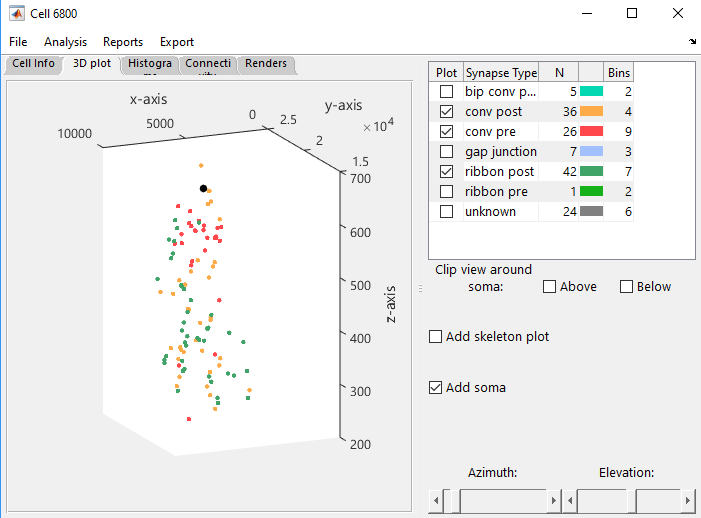
\includegraphics[width=\textwidth]{c6800_plot3}
				\vskip5pt
				AII amacrine cell synapses
			\column[]{0.5\textwidth}
				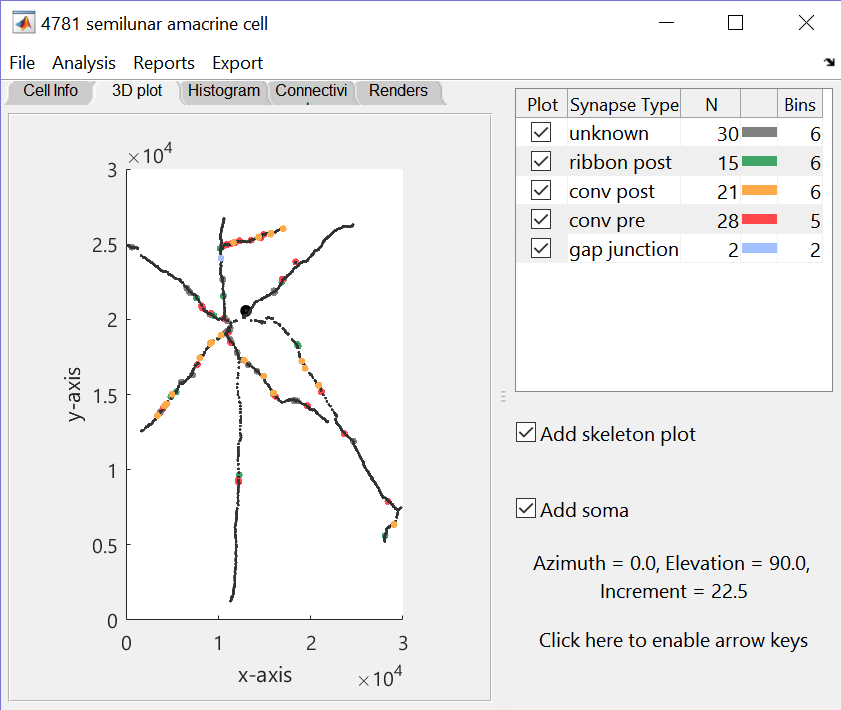
\includegraphics[width=\textwidth]{c4781_plot3}
				\vskip5pt
				Semilunar synapses \& skeleton
		\end{columns}
\end{frame}
% --------------------------------------------------- Slide --	
\subsection{Histograms}
% --------------------------------------------------- Slide --
\begin{frame}
	\frametitle{Histograms}
	\begin{columns}
		\column[]{0.5\textwidth}
			There are two histograms. These plot synapse count as a function of:
			\begin{itemize}
				\item Distance from soma
				\item Section number (z-axis)
			\end{itemize}
		Use the Synapse Table to edit the number of bins. Add the cell skeleton to see dendrite stratification.
		\column[]{0.5\textwidth}
			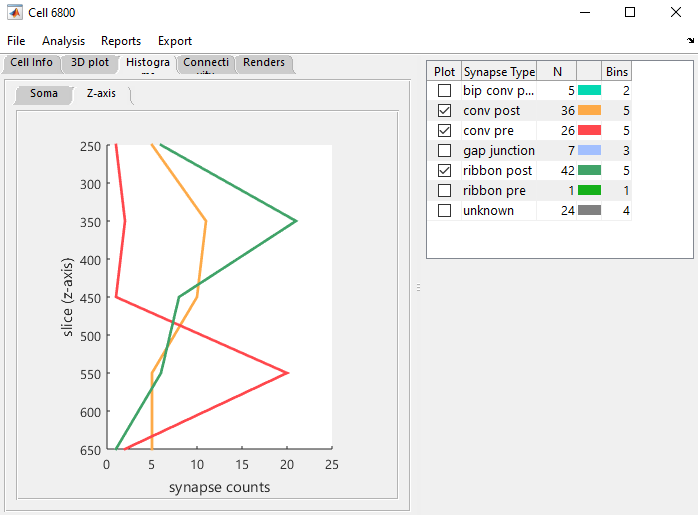
\includegraphics[width=\textwidth]{c6800_histZ}
		\vskip3pt
		Z-axis synapse distribution for a putative AII AC. This synapse asymmetry isn't news but is still good to see.
	\end{columns}
\end{frame}
% --------------------------------------------------- Slide --
\subsection{Connectivity}
\begin{frame}[fragile]
	\frametitle{Connectivity}
	To add connectivity data, save a network map in Tulip as a JSON file, as described above. Then in Matlab:
	\begin{lstlisting}[language=matlab]
c207.addConnectivity('c207hops.json');\end{lstlisting}
	\vskip10pt
	\begin{columns}
		\column[]{0.5\textwidth}
		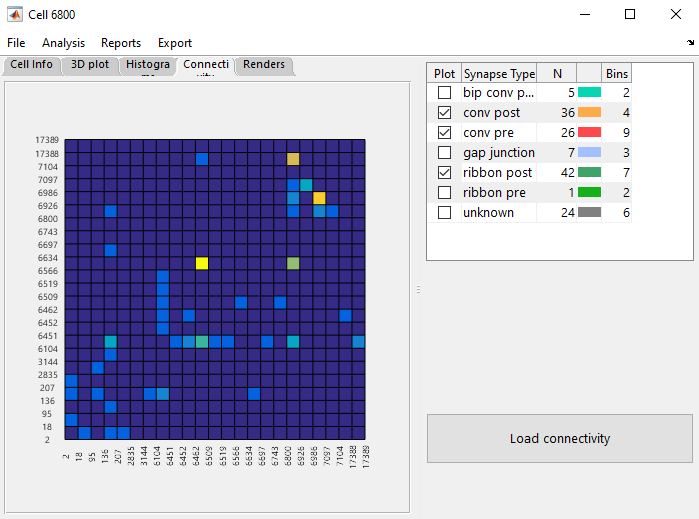
\includegraphics[height=0.4\textheight]{c6800_network}	
		\vskip10pt
		Connectivity for the AII AC.
		\column[]{0.5\textwidth}
		The connectivity matrix is weighted by the number of unique synapses between two cells (dark blue for 0 synapses). Directed synapses will only register a contact from the pre $\rightarrow$ post-synaptic neuron.
	\end{columns}
\end{frame}
% --------------------------------------------------- Slide --
\begin{frame}[fragile]
	\frametitle{Connectivity}
	The network data is split into edges and nodes, each with their own table. The tables can be exported to Excel as \texttt{.csv} or as a text file from the UI menu bar.\\
	\vskip10pt
	To print a easily readable table to the command line use the networkTable function
\begin{lstlisting}[language=matlab]
networkTable(c207);\end{lstlisting}
\end{frame}
% --------------------------------------------------- Slide --
\subsection{Images}
\begin{frame}
	\frametitle{Blender Renders and Cell Fills}
	\begin{columns}
		\column[]{0.5\textwidth}
		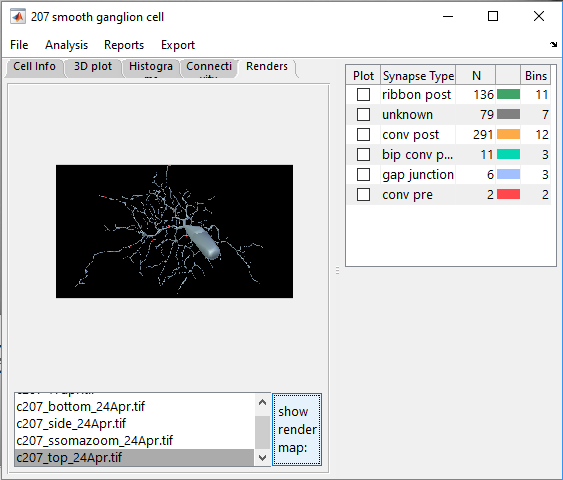
\includegraphics[width=0.9\textwidth]{c207_render}
		\hskip10pt
		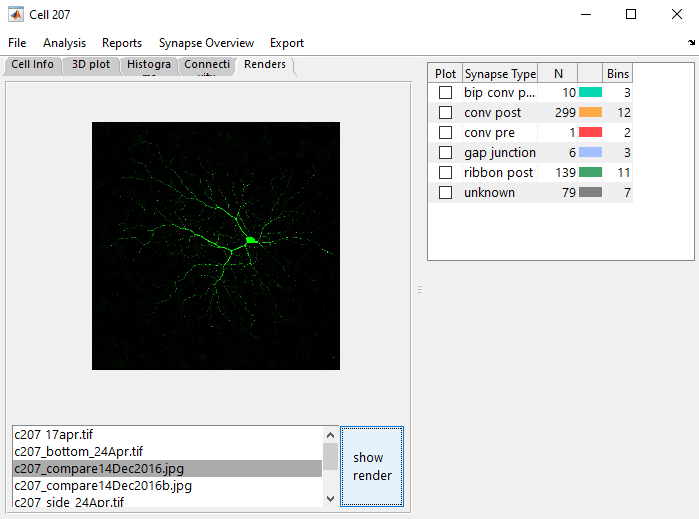
\includegraphics[width=0.9\textwidth]{c207_cellfill}
		\column[]{0.5\textwidth}
		For now, set the \texttt{renderDir} in \texttt{getFilepaths.m} to the file your images are saved into. The UI find the images if their filename includes the letter `c' followed by cell number (like `c207'). I hope to improve this at some point.
		\vskip15pt
		This isn't limited to renders and could include whatever images and diagrams are helpful. For example, I can compare my ON-smooth cell reconstructions and cell fills.
	\end{columns}
\end{frame}
% --------------------------------------------------- Slide --
\subsection{Reports}
% --------------------------------------------------- Slide --
	\begin{frame}
		\frametitle{Reports}
		This is pretty limited... Right now you can generate two reports:
		\begin{itemize} 
			\item Location IDs of unknown synapses
			\item An overview of all synapse types
		\end{itemize}
		The report name is auto-generated and will overwrite any existing reports of the same type for that neuron.\\Let me know any other reports that would be of use.
	\end{frame}
% --------------------------------------------------- Slide --
\section{Utilites}
% --------------------------------------------------- Slide --	
	\begin{frame}
		\frametitle{Save}
		Neurons do not need to be saved, as the underlying data is replaced with each update. However, if you would like to save a neuron for offline work, here's some guidelines: 
		\begin{block}{Save Cell Info}
			After adding information to the Cell Info Panel, make sure to press the button \texttt{[Add to cell info]}.\\ This saves cell attributes to the Neuron object.
		\end{block}
		\begin{block}{Save Neuron}
			To save the Neuron object itself, go to \texttt{File-->Save Cell} or save from the command line to the current directory. 
		\end{block}
	\end{frame}
% --------------------------------------------------- Slide --
\begin{frame}
	\frametitle{Export}
\end{frame}
% --------------------------------------------------- Slide --

% --------------------------------------------------- Slide --	
\begin{frame}
	\frametitle{Configuration}
		These are found in the \texttt{defaults} folder.
		\begin{enumerate}
			\item \textbf{Directories} - to save time navigating to the correct directory each time, edit \texttt{getFilepaths.m}
			\item \textbf{Cell types and subtypes} - go to \texttt{getCellTypes.m} and \texttt{getCellSubtypes.m}. Let me know if any are missing.
			\item \textbf{Synapse colors} - go to \texttt{getStructureColors.m} to change the default colors for each synapse. 
		\end{enumerate}
\end{frame}

% --------------------------------------------------- Slide --
\section{Group Analysis}
% --------------------------------------------------- Slide --
\subsection{NeuronAnalysis Class}
% --------------------------------------------------- Slide --
\begin{frame}
	\frametitle{NeuronAnalysis Class}
	The NeuronAnalysis class helps keep population data organized by managing input parameters and results of common analyses. To create a new analysis, subclass NeuronAnalysis and edit the \texttt{doAnalysis} and \texttt{visualize} methods.
	\vskip10pt
	See \texttt{Tutorial.m} for information on these existing classes:
	\begin{itemize}
		\item \textbf{DendriticFieldHull} - uses convex hull to estimate dendritic field area, includes methods for removing axons prior to analysis.
		\item \textbf{PrimaryDendriteDiameter} - returns the median dendrite diameter at a given distance from the soma.
	\end{itemize}
\end{frame}
% --------------------------------------------------- Slide --
\begin{frame}[fragile]
	\frametitle{Mosaic Class}
	The Mosaic class is a first attempt at support for groups of neurons. This allows the most important properties of each neuron to be accessed and analyzed as a group.\\
	\vskip10pt
	Mosaic is the parent class that should not be used directly. Instead use Generic or one of the cell type specific subclasses (BipolarCells, Photoreceptors, HorizontalCells). 
\end{frame}
% --------------------------------------------------- Slide --
\subsection{Mosaic Class}
% --------------------------------------------------- Slide --
\begin{frame}[fragile]
	\frametitle{Mosaic}
	These core methods are common to all Mosaic subclasses, not just Generic.
	\begin{lstlisting}[language=matlab]
% Create a Mosaic by passing a Neuron
bip = Generic(c142);
% Add a description of the mosaic
bip.describe('s-off bipolar cells');
% Add Neuron to the mosaic
bip.add(c1411);
% Remove a Neuron
bip.rmNeuron(1411); % by cell number
bip.rmRow(2); % by row number
% To view the neurons in the cmd line:
bip
% Mosaic is essentially matlab's table. To use the full range of table methods, cast to table:
T = mosaic2table(bip);
\end{lstlisting} 
\end{frame}
% --------------------------------------------------- Slide --
\begin{frame}[fragile]
	\frametitle{Mosaic Visualization}
	\begin{columns}
		\column[]{0.75\textwidth}
			The Mosaic class grew from functions designed to view the photoreceptor mosaic. Accordingly, the visualization methods are most developed.
\begin{lstlisting}[language=matlab]
% Basic plot of cell 'somas'
% Plot to existing axis
bip.somaPlot('ax', axesHandle);
% Include cell ID labels
bip.somaPlot('lbl', true);
% Set the color and linewidth
bip.somaPlot('co', [1 0 0], 'lw', 1);\end{lstlisting}
\vskip15pt
Additional cell-type specific parameters can be found in each Mosaic class' description.
		\column[]{0.25\textwidth}
			\begin{center}
				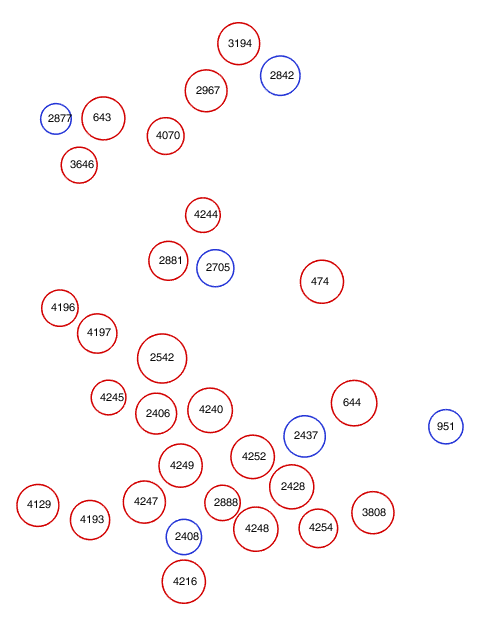
\includegraphics[width=\textwidth]{prMosaic}
				\vskip10pt
				{\footnotesize Cone mosaic with cellID labels}	
			\end{center}		
	\end{columns}
\end{frame}
% --------------------------------------------------- Slide --
\section{Appendix}
% --------------------------------------------------- Slide --
\begin{frame}
	\frametitle{Appendix}
	Here's some information and methods that are less essential:
	\begin{itemize}
		\item Links
		\item Tulip import method
		\item Will add more with next update...
	\end{itemize}
\end{frame}
% --------------------------------------------------- Slide --
\subsection{Links}
% --------------------------------------------------- Slide --
\begin{frame}
	\frametitle{Links}
	The SBFSEM-tools \href{www.github.com/sarastokes/sbfsem-tools}{\textcolor{blue}{repository}} can be found on Github.\\
	I included two open source matlab toolboxes: \href{https://www.mathworks.com/matlabcentral/fileexchange/33381-jsonlab--a-toolbox-to-encode-decode-json-files}{\textcolor{blue}{JSONLab}} and the \href{https://www.mathworks.com/matlabcentral/fileexchange/47982-gui-layout-toolbox}{\textcolor{blue}{GUI Layout Toolbox}}.\\
	The software used for annotations is \href{https://connectomes.utah.edu/}{\textcolor{blue}{Viking}}, developed by Jamie Anderson and the Marc Lab at University of Utah.\\
	Useful free programs involved in these analyses:
	\begin{itemize}
		\item \href{http://chip.de/downloads/Tulip-64-Bit_41528289.html}{\textcolor{blue}{Tulip}} supports graph visualization. The documentation for Tulip's Python package can be found \href{http://tulip.labri.fr/Documentation/4_10_0/tulip-python/html/index.html}{\textcolor{blue}{here}}.
		\item \href{http://www.blender.com}{\textcolor{blue}{Blender}} for 3D renders of neurons.
	\end{itemize}
	SBFSEM-tools was developed in the \href{http://www.neitzvision.com/}{\textcolor{blue}{Neitz lab}} at University of Washington.
\end{frame}	
% --------------------------------------------------- Slide --
\subsection{Tulip Import}
% --------------------------------------------------- Slide --
\begin{frame}[fragile]
	\frametitle{Import}
	\framesubtitle{Step One: Tulip}
	\begin{block}{}
		Open a cell in Tulip and then open the Python command line. It's on the bottom toolbar.\\
		Set the file name* and file path:
		\begin{lstlisting}[language=python]
		outputFile = "C:\...\c207.json"\end{lstlisting}
		Then run these two lines:
		\begin{lstlisting}[language=python]
		params = tlp.getDefaultPluginParameters('JSON Export', graph)
		success = tlp.exportGraph('JSON Export', graph, outputFile, params)\end{lstlisting}
	\end{block}
\end{frame}
% --------------------------------------------------- Slide --
\begin{frame}
	\frametitle{Import}
	\framesubtitle{Step One: Tulip}
	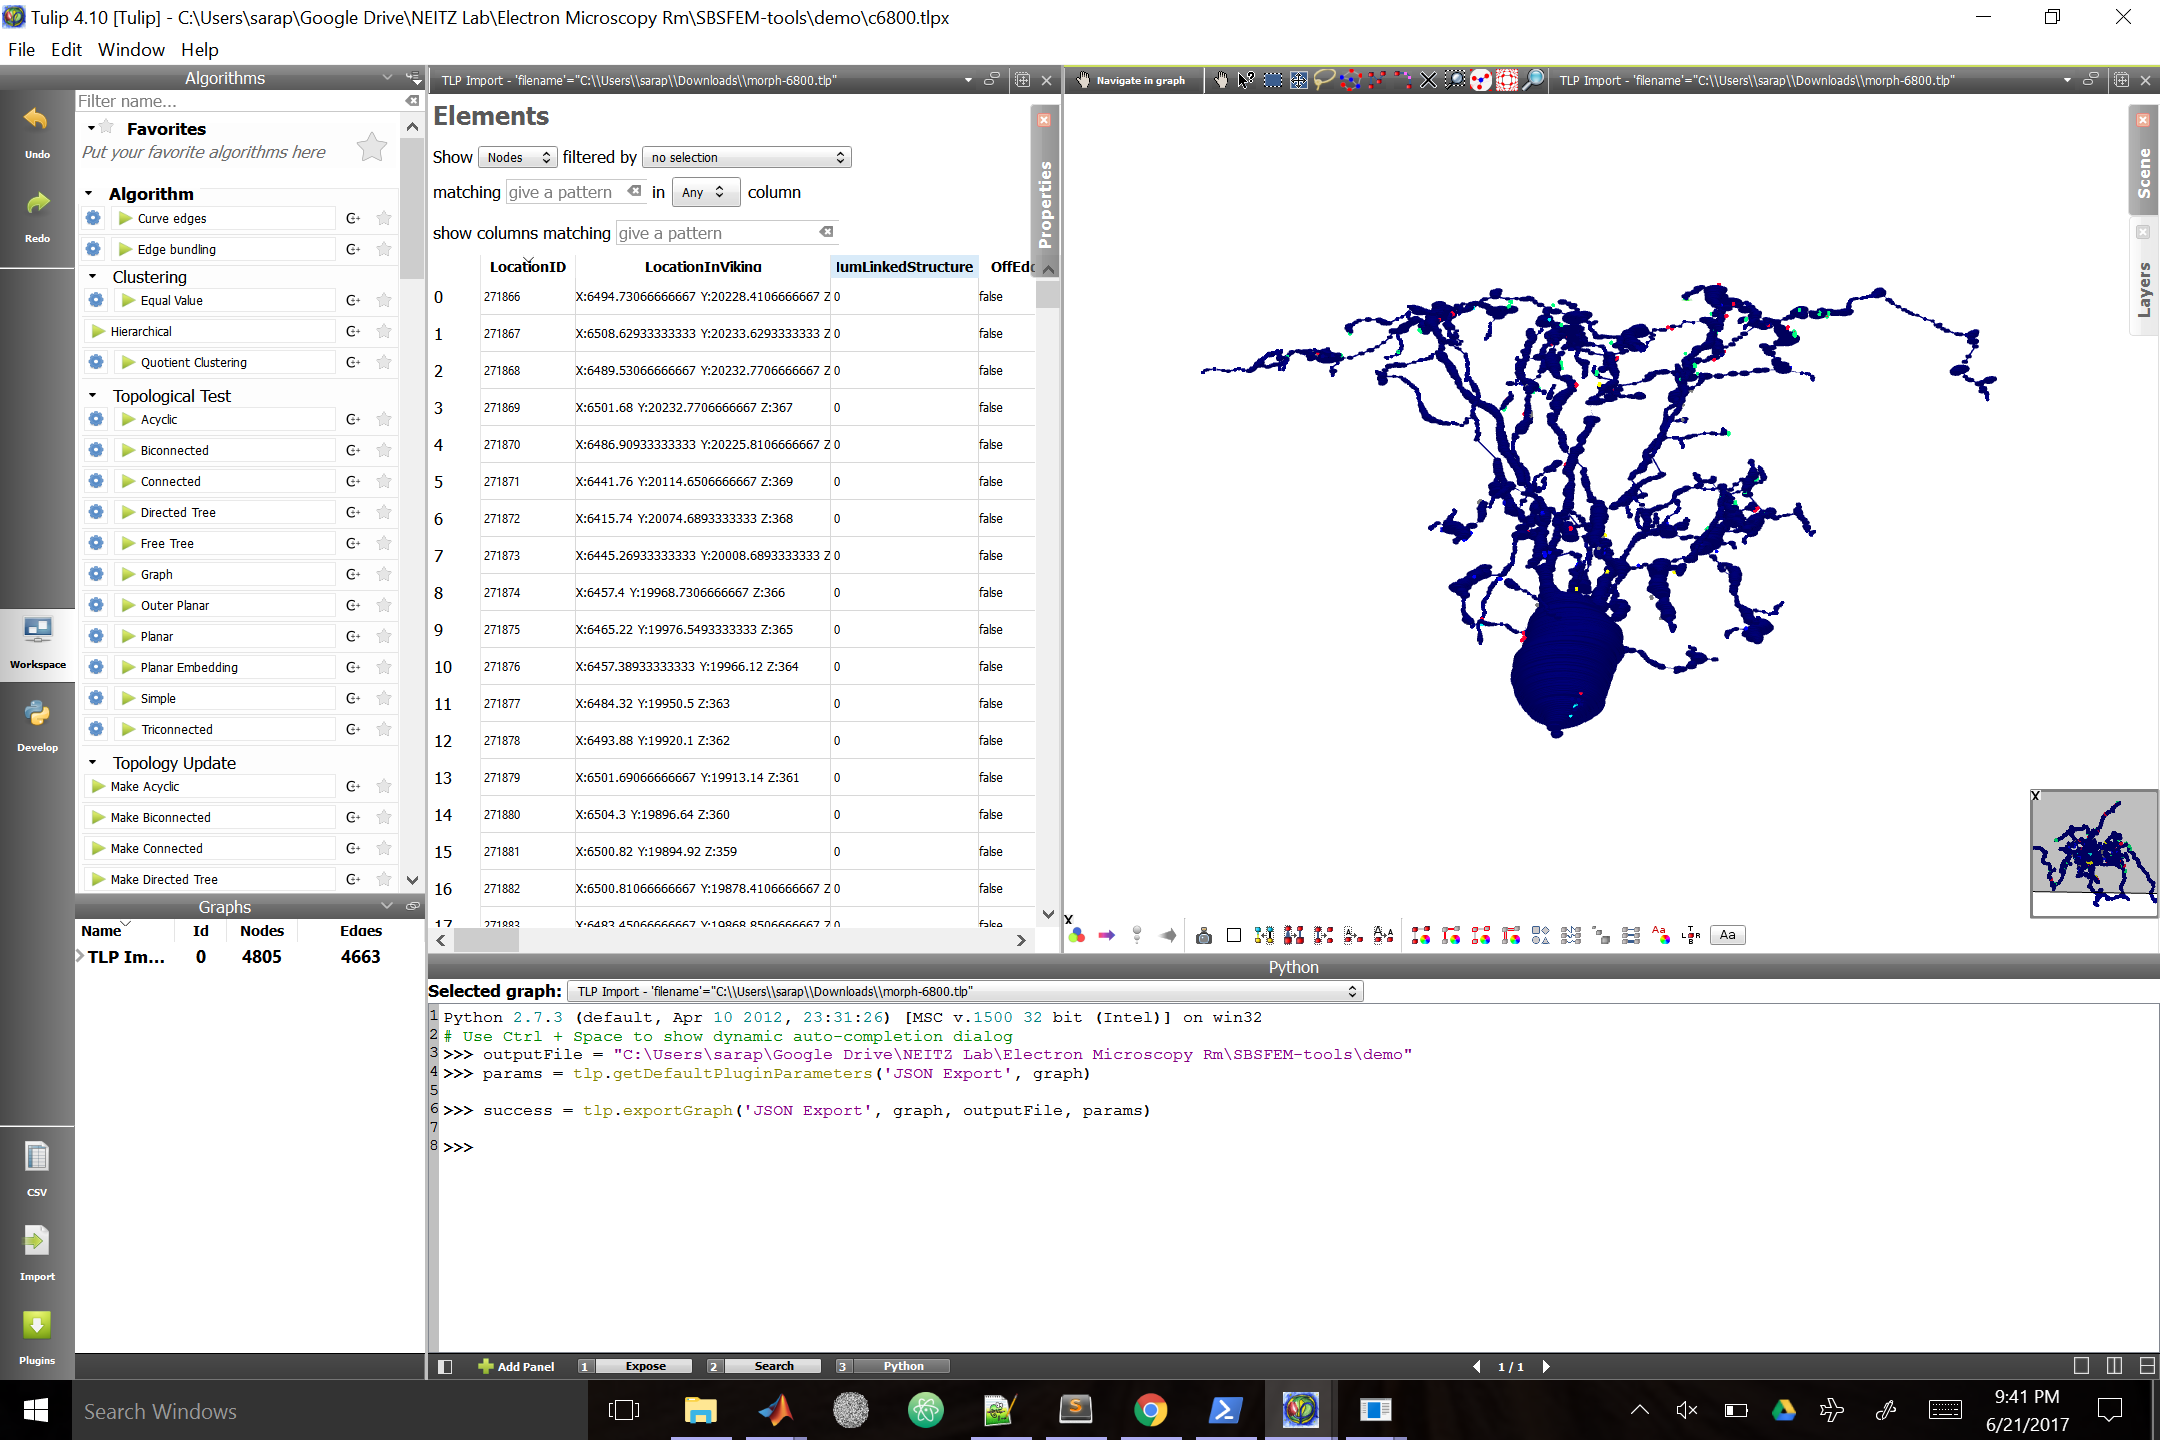
\includegraphics[width = 0.9\textwidth]{tulip_python}
\end{frame}
% --------------------------------------------------- Slide --
\begin{frame}[fragile]
	\frametitle{Alternative Streamlined Import}
	\framesubtitle{Step One - Tulip}
	If you're comfortable with Python, you can skip opening Tulip's UI entirely.\\
	First get the Tulip modules:
	\begin{lstlisting}
	$ pip install tulip-python\end{lstlisting}
	This will allow you to export \texttt{.tlp} (or compressed \texttt{.tlp.gz}) files to JSON from a command line without Tulip's UI.
	\begin{lstlisting}[language=python]
	from tulip import tlp
	graph = tlp.loadGraph("C:\...\morph-207.tlp")
	outputFile = "C:\...\c207.json"
	params = tlp.getDefaultPluginParameters('JSON Export', graph)
	success = tlp.exportGraph('JSON Export', graph, outputFile, params)\end{lstlisting}
\end{frame}
% --------------------------------------------------- Slide --
\begin{frame}[fragile]
	\frametitle{Import}
	\framesubtitle{Step Two - MATLAB}
	Load in the JSON file and create a Neuron object:
	\begin{lstlisting}[language=matlab]
	c207 = Neuron('c207.json');\end{lstlisting}
	A dialog box will ask for the cell number and source (temporal, inferior, rc1). To avoid that, include them while creating the Neuron object:
	\begin{lstlisting}[language=matlab]
	% output = Neuron(filename, cellNumber, source);
	c207 = Neuron('c207.json', 207, 'temporal');\end{lstlisting}
	To update the underlying data for an existing Neuron:
	\begin{lstlisting}[language=matlab]
	c207.updateData('c207.json');\end{lstlisting}
	Open up the user interface:
	\begin{lstlisting}[language=matlab]
	c207.openUI;\end{lstlisting}
\end{frame}
% --------------------------------------------------- Slide --
\end{document}